\title{G54RFP Coursework Part II}
\author{
  Jack Ellis \\
  psyje5@nottingham.ac.uk\\
  4262333
}
\date{}
\documentclass[12pt]{article}
\usepackage{graphicx}
\graphicspath{ {Images/} }
\usepackage{mathtools}
\usepackage {listings}
\lstset{
  breakatwhitespace=false,
  language=Haskell,
  basicstyle=\ttfamily\small,
  showstringspaces=false,
  xleftmargin=-0.1\textwidth,
  xrightmargin=-0.1\textwidth
}

\begin{document}
\maketitle
\tableofcontents

\section{Task II.1 - Dining Philosophers}

\lstinputlisting[firstline=5,lastline=6]{../Philosophers/Phils.hs}

For clarity, I firstdefined a pair of new types: \verb|Spoon| and \verb|Philosopher|, which map to \verb|TMVar Int| and \verb|String| respectively.
In my implementation the Philosophers are eating with spoons, in order to avoid confusion between forks (the cutlery) and forks (the making of new threads).
I then defined 3 functions to initialise, take, and return spoons.

\lstinputlisting[firstline=11,lastline=18]{../Philosophers/Phils.hs}

These are essentially simple maps of the STM Monad's functions to relate them to the \verb|Spoon| type.

\lstinputlisting[firstline=20,lastline=25]{../Philosophers/Phils.hs}

I elected to use lecturers in the School of Computer Science as my philosopher names.

\lstinputlisting[firstline=27,lastline=41]{../Philosophers/Phils.hs}

Now for "running a philosopher".
This is the infinite process by which they become hungry, get both spoons, eat, return both spoons, think, and become hungry again.
This requires both spoons to be available, consequently we try to get both the left and right spoons \verb|atomically|, ensuring that the process will halt until both are available.
The thread is then delayed by a random amount between 1 and \verb|maxDelay| (currently 5) seconds while the philosopher eats, and upon that being completed the spoons are \verb|atomically| returned.
Another delay of between 1 and \verb|maxDelay| seconds, and the process runs again with the same arguments.

\lstinputlisting[firstline=43,lastline=46]{../Philosophers/Phils.hs}

Before \verb|main| is declared we need a function to make pairs of \verb|Spoon|s, for passing into the \verb|runPhil| function.
This is relatively trivial.

\lstinputlisting[firstline=48,lastline=58]{../Philosophers/Phils.hs}

Finally, \verb|main|, where everything is put together.
First we generate a list of spoons equal to the length of the list of philosophers (whose names we print to the screen).
Then we declare 3 variables:
\begin{itemize}
  \item \verb|namedPhils|, which is a list of partially applied \verb|runPhil|s waiting for the \verb|(l,r)| argument.
  \item \verb|spoonPairs|, which is a list of pairs of \verb|Spoon|s generated from the list of \verb|Spoon|s generated earlier.
  \item \verb|philsWithSpoons| is then the result of zipping \verb|namedPhils| with \verb|spoonPairs|, the list of functions to be forked.
\end{itemize}

Finally \verb|mapM_| is used to fork all of the \verb|philsWithSpoons| processes, taking only their side-effects (namely the printing).
The \verb|getLine| at the end is used to stop the function, and it \verb|return|s empty.
\par
In the \verb|Philosophers| folder containing the source code is a file \verb|output.txt| containing 65 lines of program output; the following is the first 15 lines from that file (not including the list of philosophers and "Press enter to stop" message).

\lstinputlisting[firstline=3,lastline=17]{../Philosophers/output.txt}

\subsection{This approach versus the \textit{Resource Hierarchy Solution}}
In the \textit{Resource Hierarchy Solution}, the resources (spoons) are given an order of priority, and  of the two required, each "unit of work" (philosopher) will only attempt to access the lower-numbered one first.
The main issue with this approach is that if the first four philosophers are to pick up their lower spoon, the fifth cannot, and a deadlock occurs.
The STM approach avoids this; by not enforcing which spoon is picked up first and only requiring that both spoons are picked up at some point before eating can begin it ensures that no such deadlock can occur.

\subsection{This approach versus the \textit{Arbitrator Solution}}
In the \textit{Arbitrator Solution}, an additional entity is introduced: a waiter who must be asked before any philosopher can pick up a spoon, and who gives permission to one philosopher at a time until that philosopher has picked up both spoons.
The main issue with this approach is the introduction of an additional entity (and the increased complexity associated with that), and the fact that it can result in reduced parallelism; if one philosopher is eating and a neighbour requests a spoon, no other philosophers can even request their own spoons.


\pagebreak


\section{Task II.2 - Threepenny Calculator}

\subsection{Parsing a String to a Maybe Float}

Firstly I define a couple of data types, \verb|Calc|, and \verb|Op|. These will form the basis of the overall calculator and the shunting-yard algorithm, respectively.

% DEFINING CALC
\lstinputlisting[firstline=7, lastline=9]{../Calculator/calculator.hs}

\verb|working| refers to the working space; the string denoting the equation that, upon the user hitting '=', will be evaluated.
I elected to model my calculator on a scientific model because I find them more intuitive to use than the traditional kind, as well as the fact that it is essentially an example of lazy evaluation; computation only occurs when the answer is demanded, a la Haskell itself.
\verb|ans| refers to the answer to the previous equation, and is the space where upon evaluation the result of the equation described in \verb|working| will be stored.
\verb|mem| is the calculator's memory; slightly unnecessary here given the answer recall function afforded by \verb|ans| however any Float value can be stored here.

% DEFINING OP
\lstinputlisting[firstline=11,lastline=13]{../Calculator/calculator.hs}

Here the \verb|symbol| element is the symbol of the operator, used for lookup purposes.
The \verb|precedence| is the precedence of the operator; this follows BODMAS rules and the values are arbitrary.
\verb|associativity| is used for Shunting-Yard: one of the things that the algorithm checks is the associativity of the operator at the top of the stack, so that gets stored here.

% DEFINING USEFUL GLOBALS
\lstinputlisting[firstline=18, lastline=24]{../Calculator/calculator.hs}

These two are used in the Threepenny section; \verb|errorMsg| gives a consistent message when something errors out, and is used for equality, and \verb|emptyCalc| is used on initialisation and when a user hits the 'C' button.

% DEFINING LISTS OF OPS, FNS, AND SPECIALS
\lstinputlisting[firstline=29, lastline=43]{../Calculator/calculator.hs}

Here the lists of operators, functions, and special values are defined; these are defined such that the Shunting-Yard algorithm can detect whether or not a token it encounters is an operator (and if it is the precedence and associativity associated with it), a function, or a special value (currently only pi).

% DEFINING HELPERS DOWN TO SPECIALCONVERT
\lstinputlisting[firstline=45, lastline=61]{../Calculator/calculator.hs}

Now some helper functions to check whether or not a token is an operator, and get an operator's precedence or associativity.
Also a function to check whether or not a token is a function, and whether or not one is a special value and convert that token to its actual value.

%DEFINING PARSEEQN, PARSEEQN', AND PARSEEQN''
\lstinputlisting[firstline=63, lastline=88]{../Calculator/calculator.hs}

Now we define a series of functions that take a string and convert it into Reverse Polish Notation (RPN).
\verb|parseEqn| is effectively a setup function which takes the string, separates it by the delimiter (in this case spaces), and passes that and an empty tuple through to \verb|parseEqn'|.
In terms of \verb|parseEqn'|, if it reaches the end of the list of strings it will return the output plus the operator stack.
If it has tokens to evaluate, it has 4 options: if that token is an operator it will go to another helper function to determine where in the \verb|(output, stack)| tuple it fits.
This will be discussed later.
If the token is a function it is cons'ed to the stack, and if it is a value (numeric or special) is is appended to the output.
\verb|parseEqn''| adds tokens to the stack in accordance with Shunting-Yard rules, which have been minimised somewhat.

% DEFINING EVALRPN, SAFEEVAL1, SAFEEVAL2, AND SAFEREAD
\lstinputlisting[firstline=90, lastline=130]{../Calculator/calculator.hs}

Finally for the "evaluating a string" section of the program, a safe evaluator of Reverse Polish Notation.
\verb|safeEvalRPN| does the overall evaluation of the RPN list of tokens to a Maybe Float.
\verb|safeEval1| and \verb|2| are the safe evaluators for unary and binary functions respectively, and \verb|safeRead| is a safe reader for \verb|String|s to \verb|Float|s.

% SAFEDO
\lstinputlisting[firstline=132, lastline=133]{../Calculator/calculator.hs}

Finally \verb|safeDo| composites \verb|safeEvalRPN| and \verb|parseEqn|.

\subsection{Applying this to Threepenny GUI}

% DEFINING BTNS
\lstinputlisting[firstline=139, lastline=143]{../Calculator/calculator.hs}

The main UI component here is \verb|btns|, which is a list of tuples containing \verb|UI Element|s and functions which take an \verb|Element| and return an \verb|Event|.
This will be used for showing the buttons, as well as binding them to the \verb|Calc -> Calc| functions.
The structure of the list is representative of the layout of the page, and \verb|(UI.br, id)| tuples are used for line breaks.

% DEFINING BUTTON HELPERS
\lstinputlisting[firstline=183, lastline=198]{../Calculator/calculator.hs}

All of the above could have been incoroporated into a \verb|where| clause in the \verb|btns| declaration, but for clarity's sake I thought it best to define them separately, with their type signatures.
\verb|newButton| and \verb|makeEvent| are functions that take a string and return a button with that string as a label, and make an event out of some variable given to it respectively.
They are used in \verb|btns| for easy generation of buttons and associated events.
\verb|calcNeg| is used to make the value stored in 


% DEFINING CALCUPDATEWORKING
\lstinputlisting[firstline=200, lastline=209]{../Calculator/calculator.hs}

\verb|calcUpdateWorking| updates the working space of the calculator; if the value being added is an operator and the space is currently empty it will perform that operator on the current answer value.
If the working space is occupied by an error message, it will be overwritten and ignored.
Otherwise the new token will be appended to the working space.

% DEFINING CALCEVAL
\lstinputlisting[firstline=211, lastline=215]{../Calculator/calculator.hs}

\verb|calcEval| takes the \verb|Calc| and, using the string evaluator defined above, updates it based on the contents of the working space.
If the result of evaluating it is \verb|Nothing| it will print an error message to the screen, otherwise it will have the correct value in the answer space and allow the user to input more.

% DEFINING SETUP
\lstinputlisting[firstline=217, lastline=232]{../Calculator/calculator.hs}

\verb|setup| sets up the FRP elements, drawing the buttons, marrying buttons with the functions they call, and drawing the workspace and answer sections.

% DEFINING MAIN
\lstinputlisting[firstline=234, lastline=237]{../Calculator/calculator.hs}

Finally, \verb|main| sets up the whole thing and starts the web server.

\subsection{The Calculator In Action}

In figure \ref{fig:startup} we can see the calculator on a fresh page open.
The buttons function as expected by and large, numbers and functions appending to the working space, the \verb|Ans| key appending to it the value currently stored in the main \verb|Calc| variable's \verb|ans| record (displayed just below the working space.
The memory buttons work as follows:
\begin{itemize}
  \item \verb|M+|: sets the memory to the current answer value.
  \item \verb|M|: appends the current memory value to the working space.
  \item \verb|MC|: clears the memory (sets it to 0).
\end{itemize}

\verb|C| and \verb|CE| do not affect the memory value; this is persistent until the user either closes the calculator or clears it.

Figure \ref{fig:inuse} shows the calculator in the middle of being used.
Here the working space contains \verb|sin(5)|, and the answer value is \verb|101.0|.
The value of the working space will not be passed into the answer field until the user presses the \verb|=| button.

If the working space is empty and the user inputs an operator, that operator will take as its first argument the current answer value, i.e. if the working space was empty in figure \ref{fig:inuse} and I hit the \verb|-| key the working space would then read \verb|101.0-|.

Figure \ref{fig:error} shows the calculator before and after attempting to evaluate an invalid expression; this one has mismatched brackets, however the calculator will return this error message on any poorly-formed equation (i.e. multiple operators without numbers in between).
If a user then adds to the working space the error message is automatically overwritten and calculation can continue as normal.

\begin{figure}[ht]
\centering
\caption{The calculator as it starts up}
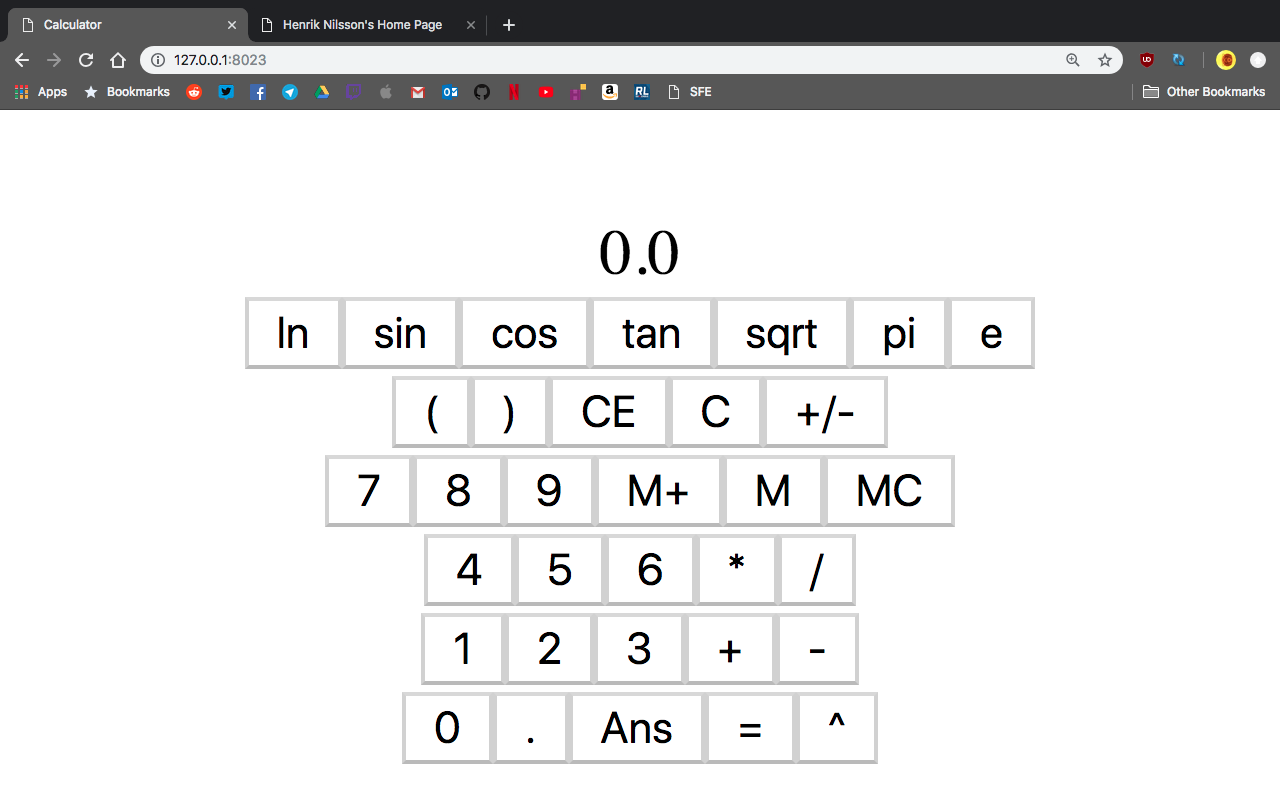
\includegraphics[width=0.5\textwidth]{01.png}
  \label{fig:startup}
\end{figure}

\begin{figure}[ht]
\centering
\caption{The calculator in use}
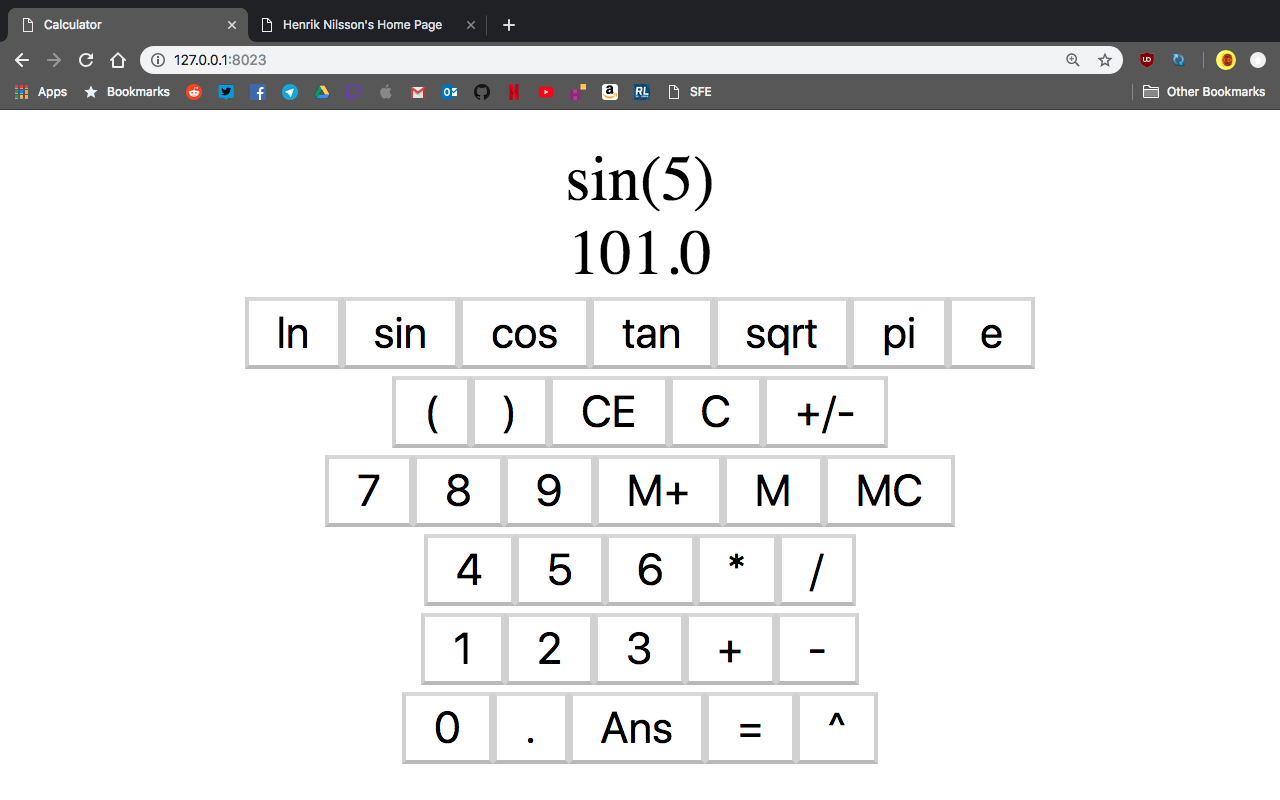
\includegraphics[width=0.5\textwidth]{02.png}
  \label{fig:inuse}
\end{figure}

\begin{figure}[ht]
\centering
\caption{The calculator with an invalid expression in the working space, and the result of pressing equals}
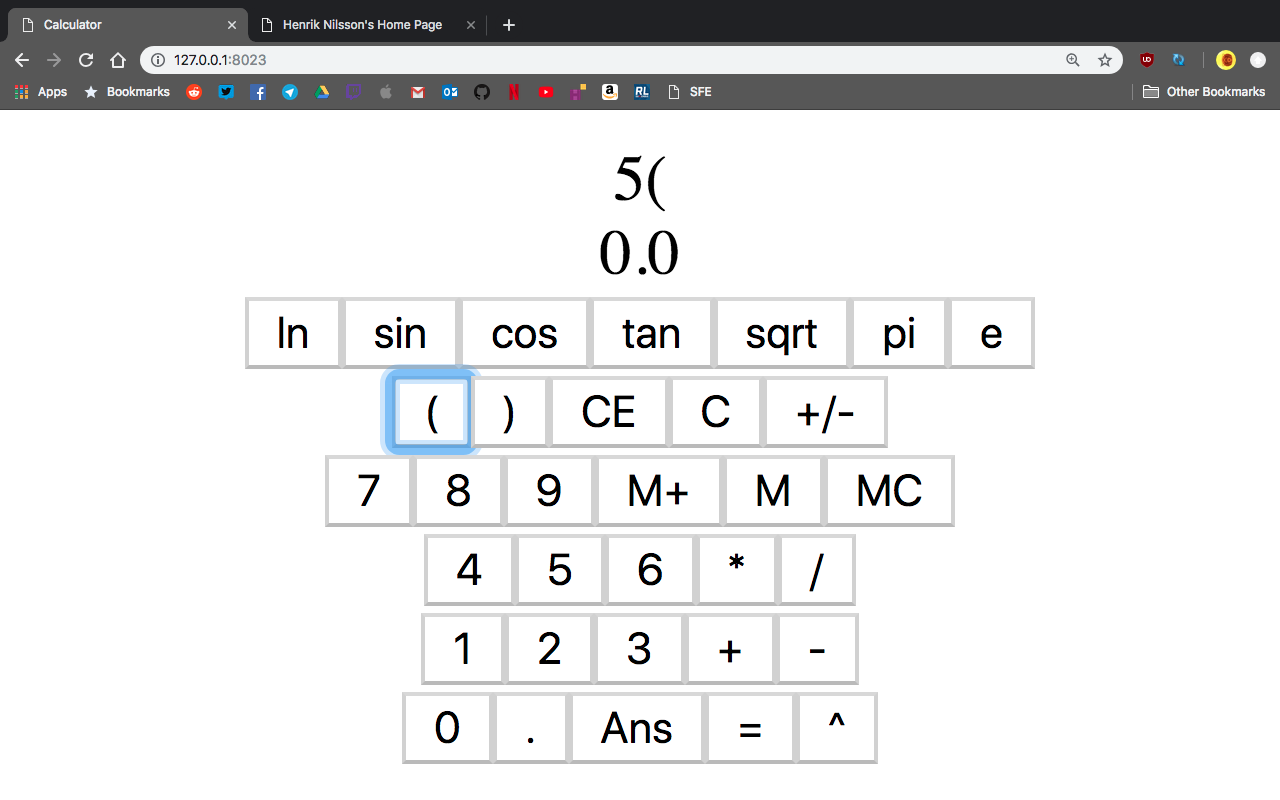
\includegraphics[width=0.5\textwidth]{03-1.png}
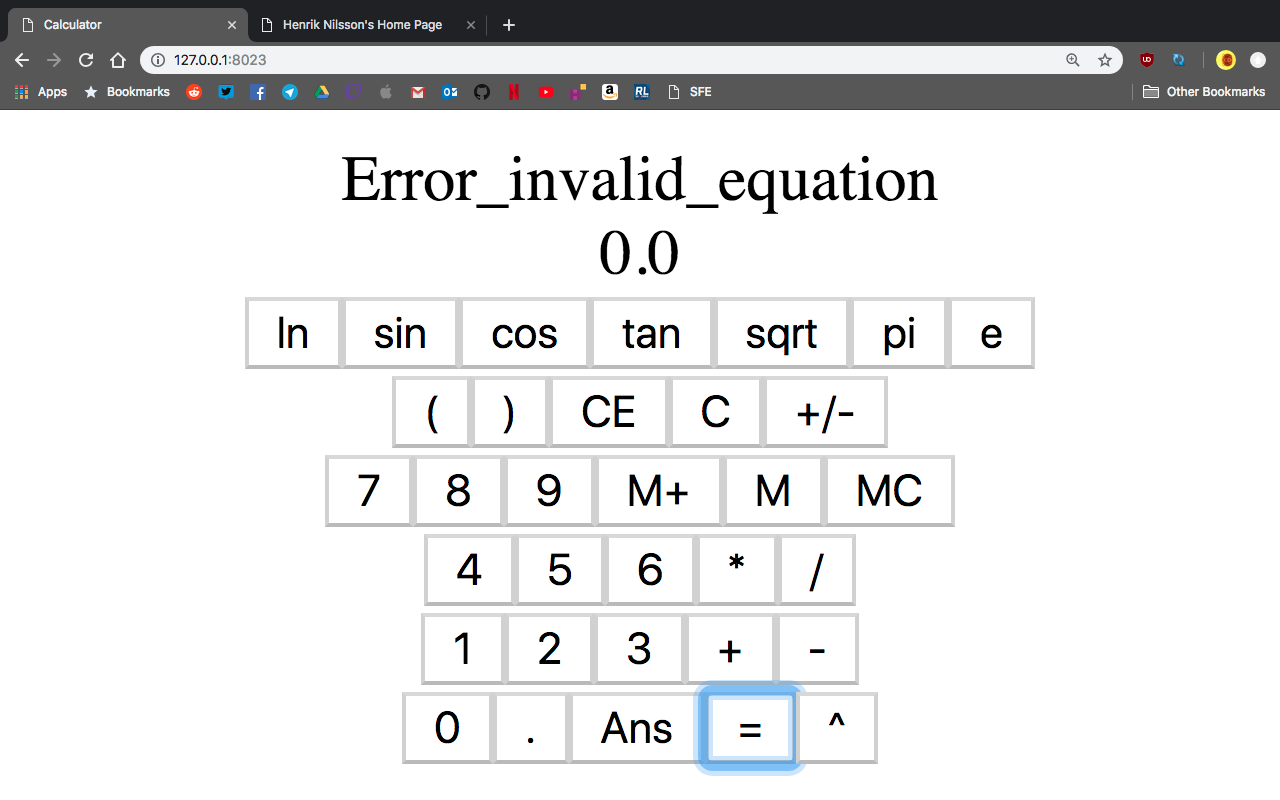
\includegraphics[width=0.5\textwidth]{03-2.png}
  \label{fig:error}
\end{figure}

\end{document}
